% Options for packages loaded elsewhere
\PassOptionsToPackage{unicode}{hyperref}
\PassOptionsToPackage{hyphens}{url}
%
\documentclass[bachelor,openany,oneside,color]{buaathesis}
\usepackage{cjkindent}
\usepackage{gbt7714}
\usepackage{amsmath}
\citestyle{numerical}
\usepackage{lmodern}
\usepackage{amssymb,amsmath}
\usepackage{ifxetex,ifluatex}
\ifnum 0\ifxetex 1\fi\ifluatex 1\fi=0 % if pdftex
  \usepackage[T1]{fontenc}
  \usepackage[utf8]{inputenc}
  \usepackage{textcomp} % provide euro and other symbols
\else % if luatex or xetex
  \usepackage{unicode-math}
  \defaultfontfeatures{Scale=MatchLowercase}
  \defaultfontfeatures[\rmfamily]{Ligatures=TeX,Scale=1}
\fi
% Use upquote if available, for straight quotes in verbatim environments
\IfFileExists{upquote.sty}{\usepackage{upquote}}{}
\IfFileExists{microtype.sty}{% use microtype if available
  \usepackage[]{microtype}
  \UseMicrotypeSet[protrusion]{basicmath} % disable protrusion for tt fonts
}{}
\makeatletter
\@ifundefined{KOMAClassName}{% if non-KOMA class
  \IfFileExists{parskip.sty}{%
    \usepackage{parskip}
  }{% else
    \setlength{\parindent}{0pt}
    \setlength{\parskip}{6pt plus 2pt minus 1pt}}
}{% if KOMA class
  \KOMAoptions{parskip=half}}
\makeatother
\usepackage{xcolor}
\IfFileExists{xurl.sty}{\usepackage{xurl}}{} % add URL line breaks if available
\IfFileExists{bookmark.sty}{\usepackage{bookmark}}{\usepackage{hyperref}}
\hypersetup{
  hidelinks,
  pdfcreator={LaTeX via pandoc}}
\urlstyle{same} % disable monospaced font for URLs
\usepackage{longtable,booktabs}
% Correct order of tables after \paragraph or \subparagraph
\usepackage{etoolbox}
\makeatletter
\patchcmd\longtable{\par}{\if@noskipsec\mbox{}\fi\par}{}{}
\makeatother
% Allow footnotes in longtable head/foot
\IfFileExists{footnotehyper.sty}{\usepackage{footnotehyper}}{\usepackage{footnote}}
\makesavenoteenv{longtable}
\usepackage{graphicx}
\makeatletter
\def\maxwidth{\ifdim\Gin@nat@width>\linewidth\linewidth\else\Gin@nat@width\fi}
\def\maxheight{\ifdim\Gin@nat@height>\textheight\textheight\else\Gin@nat@height\fi}
\makeatother
% Scale images if necessary, so that they will not overflow the page
% margins by default, and it is still possible to overwrite the defaults
% using explicit options in \includegraphics[width, height, ...]{}
\setkeys{Gin}{width=\maxwidth,height=\maxheight,keepaspectratio}
% Set default figure placement to htbp
\makeatletter
\def\fps@figure{htbp}
\makeatother
\setlength{\emergencystretch}{3em} % prevent overfull lines
\providecommand{\tightlist}{%
  \setlength{\itemsep}{0pt}\setlength{\parskip}{0pt}}
\renewcommand {\thetable} {\thechapter{}-\arabic{table}}
\renewcommand {\thefigure} {\thechapter{}-\arabic{figure}}

\author{}
\date{}

\begin{document}
\pagestyle{mainmatter}
% !Mode:: "TeX:UTF-8"

% 学院中英文名,中文不需要“学院”二字
% 院系英文名可从以下导航页面进入各个学院的主页查看
% http://www.buaa.edu.cn/xyykc/index.htm
\school
{}{}

% 专业中英文名
\major
{}{}

% 论文中英文标题
\thesistitle
{数学规划模型相关问题}

% 作者中英文名
\thesisauthor
{}{}
\titlech
\tableofcontents

\hypertarget{header-n2}{%
\title{数学规划模型相关问题}\label{header-n2}}
\mainmatter
\hypertarget{header-n7}{%
\chapter*{引言}\label{header-n7}}\addcontentsline{toc}{chapter}{引言}
\setcounter{table}{0}\setcounter{figure}{0}数学规划模型一般来讲是指优化问题模型。优化问题的三要素是决策变量,目标函数,约束条件。对优化问题来说最为关键的就是要准确地用数学公式表达出这三要素,然后利用相关的数学软件来进行求解便是操作性的问题了。

对现实世界实际问题的建模过程中,我们往往会发现要严格按照现实情况建立相关等式或不等式是非常难的,比如我们比较容易确定问题中的具体变量是哪些,但对相关约束条件的抽离则是比较麻烦,此时需要建立一些理想化的前提和基本假设,从而方便我们对三要素的建立。可以预见的是,优化问题模型的求解往往与真实状况有一定的差异,但这并不影响理想模型对现实情况的参考价值。

然而,在求解的过程中我们又会发现其他的问题:如果没有完全符合所有约束条件的解时,该如何取舍约束条件的放宽或限制?解空间对某些约束条件的影响非常敏感,而对另一些约束条件相对来说又比较``迟钝'',如何分析这些敏感性出现的原因?会不是我们的前提假设出现了问题,以及,如何由这些敏感性来更好的设计解决方案?在本次数学规划模型的应用中,我们再一次地感受到了实际问题的复杂性以及对各种条件取舍的困难程度,并积累了相关的经验,我们认为理想化的模型求解对相当一部分实际问题都是有意义的。

具体地,数学规划模型可以分为离散或连续的,或者是有约束条件的与无约束条件的,以及线性规划与非线性规划、整数规划。从难度上来讲,有约束条件的优化问题更难,非线性规划较线性规划更难。本文中涉及的数学规划模型都属于有约束条件的数学规划问题。

\hypertarget{header-n12}{%
\chapter*{摘要}\label{header-n12}}\addcontentsline{toc}{chapter}{摘要}
\setcounter{table}{0}\setcounter{figure}{0}本文中出现的四个数学模型规划问题,除最后一题外,其他三题在相关约束条件及必须的前提假设下,都得到了相应的解。训练题2是典型的01规划问题,我们通过建立相应的矩阵来求解;训练题4是整数规划问题,利用了PYTHON中的PULP库来进行求解,并且有添加一个约束条件后的问题求解,我们可以看到约束条件对解结构的不同影响。训练题6则是较为典型的线性规划问题,其难点在于对问题的简化,忽略了给出的数学表达式中的一部分,从而简化了求解;训练题13在给定的约束条件下无解,于是我们需要选择性地放宽其中的某些约束条件来取得可行解,并且尽量靠近给定约束条件,尽量符合目标函数要求。

\hypertarget{header-n14}{%
\chapter{1 训练题2}\label{header-n14}}
\setcounter{table}{0}\setcounter{figure}{0}
\hypertarget{header-n15}{%
\section{1.1 问题表述}\label{header-n15}}

一家出版社准备在某市建立两个销售代理点,向七个区的大学生售书,每个区的大学生数量表示如图,每个销售代理点只能向本区和一个相邻区的大学生售书,这两个销售代理点应该建在何处,才能使所能供应的大学生数量最大?

\begin{figure}
\centering
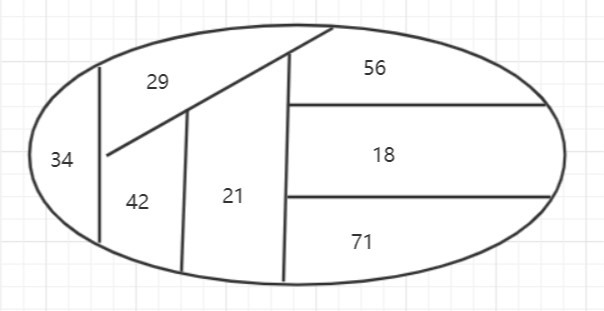
\includegraphics{D:/code/2020_course_project/math_modeling_2/pic/pc1.jpg}
\caption{}
\end{figure}

\hypertarget{header-n18}{%
\section{1.2 基本假设}\label{header-n18}}

\begin{enumerate}
\def\labelenumi{\arabic{enumi}.}
\item
  每个区的学生数量稳定,不会有新增和减少;
\item
  每个区的间隔严格按照图示的方式存在,销售点销售的区必须是本区和与本区有公共边的区;
\item
  在本市中建立两个销售点,每个销售点向两个区供书;
\end{enumerate}

\hypertarget{header-n26}{%
\section{1.3 模型建立}\label{header-n26}}

在七个区中选取两个相邻的区,并使得其四个区的大学生综合最大。将相邻的两个区的大学生数量作为一个整体看待,建立数学规划的模型。

\begin{enumerate}
\def\labelenumi{\arabic{enumi}.}
\item
  首先将七个区按如图序号进行编号:

  \begin{figure}
  \centering
  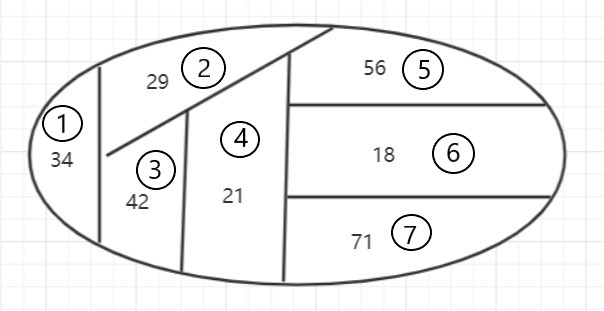
\includegraphics{D:/code/2020_course_project/math_modeling_2/pic/pc2.jpg}
  \caption{}
  \end{figure}
\item
  将相邻的两个区作为一个整体进行处理,求出学生人数的总和,将七个区变换求得的人数放入一个7
  ×
  7的矩阵之中。在矩阵的处理中(i,j)坐标当i,j的对应区相邻时,所对应的值为第i区和第j区的学生人数总和;同时当i,j区不相邻时,将矩阵对应的值设为0;同时为了避免重复处理数据,仅处理右上角区域的数据,而将左下角的数据设为0.矩阵c如图所示:
\end{enumerate}

\begin{longtable}[]{@{}cccccccc@{}}
\toprule
position1\textbackslash2 & p1 & p2 & p3 & p4 & p5 & p6 &
p7\tabularnewline
\midrule
\endhead
p1 & 0 & 63 & 76 & 0 & 0 & 0 & 0\tabularnewline
p2 & 0 & 0 & 0 & 50 & 85 & 0 & 0\tabularnewline
p3 & 0 & 0 & 0 & 63 & 0 & 0 & 0\tabularnewline
p4 & 0 & 0 & 0 & 0 & 77 & 39 & 93\tabularnewline
p5 & 0 & 0 & 0 & 0 & 0 & 0 & 0\tabularnewline
p6 & 0 & 0 & 0 & 0 & 0 & 0 & 0\tabularnewline
p7 & 0 & 0 & 0 & 0 & 0 & 0 & 0\tabularnewline
\bottomrule
\end{longtable}

\begin{enumerate}
\def\labelenumi{\arabic{enumi}.}
\item
  根据此矩阵即求解矩阵中两个值的和的最大值;同时应当满足约束条件:选取的两个矩阵点的坐标(x1,y1)与(x2,y2)中x1,x2,y1,y2各不相同。
\item
  因此在求解中,引入与数据有相同规模尺寸的01变量x矩阵来处理模型,解决问题的相关约束条件,将矩阵的纵向坐标为i,横向坐标为j:\\
  -选取四个城市对应选取矩阵中两个点:\(\displaystyle \sum^7_{i}\sum^7_{j}{x}=2\)
\end{enumerate}

-保证选取点的坐标对应城市不重复:\(\displaystyle \sum^7_{j}{x}<=1\)
,且对任意i,j,k有 x(i,j)+x(j,k)\textless=1

-问题目标函数为:max(\(\displaystyle \sum^7_{i}\sum^7_{j}{x*c}\))

\hypertarget{header-n114}{%
\section{1.4 模型求解}\label{header-n114}}

按照上述约束条件对问题进行求解,并利用Lingo处理上述模型得到最终结论,代码文件位于code文件夹的Promblem2.lg4中:

\begin{figure}
\centering
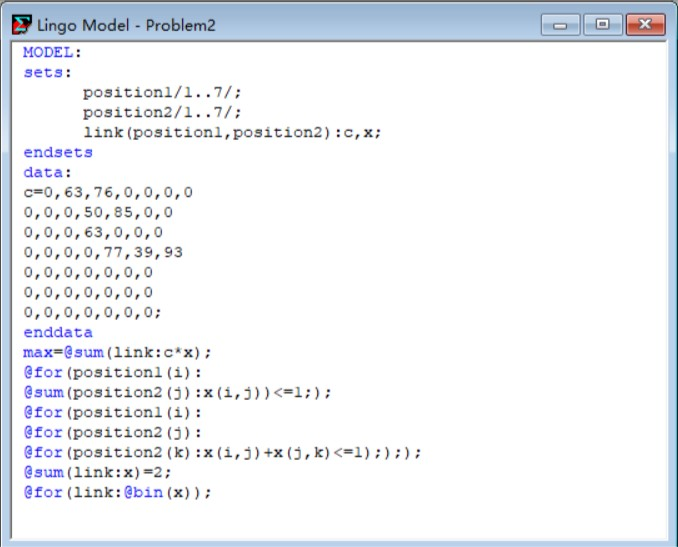
\includegraphics{/pic/pc3.jpg}
\caption{}
\end{figure}

\hypertarget{header-n117}{%
\section{1.6 结果}\label{header-n117}}

最后通过lingo求解得到,目标函数的最大值为178,在取得此值的条件下01变量x(2,5)与x(4.7)分别取值为1,其余x(i,j)=0当((i,j)
≠(2,5)(4,7)。

\begin{figure}
\centering
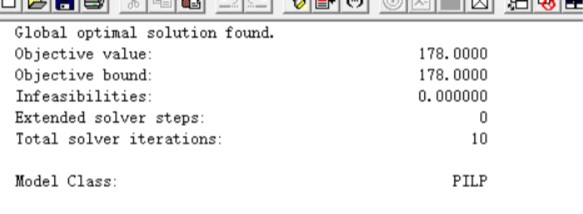
\includegraphics{D:/code/2020_course_project/math_modeling_2/pic/pc4.jpg}
\caption{}
\end{figure}

对应在实际问题中,第一个销售代理点放置在2区或5区并为2、5区供应,第二个销售代理点放置在4区或7区并为4,7区供应可以得到最大的供应学生数量178。

\hypertarget{header-n121}{%
\chapter{2 训练题4}\label{header-n121}}
\setcounter{table}{0}\setcounter{figure}{0}
\hypertarget{header-n122}{%
\section{2.1 问题表述}\label{header-n122}}

在甲乙双方的一场战争中,一部分甲方部队被乙方部队包围长达4个月。由于乙方封锁了所欲水陆交通通道,被包围的甲方部队只能依靠空中交通维持供给。运送4个月的供给分别需要2次,3次,3次,4次飞行。每次飞行编队由50架飞机组成(每架飞机需要3名飞行员),可以运送\(10^5t\)物资。每架飞机每个月只能飞行一次,每名飞行员每个月也只能飞行一次。在执行完运输任务后的返回途中有20\%的飞机会被乙方部队击落,相应的飞行员也因此牺牲或失踪。在第1个月开始时,甲方拥有110架飞机和330名熟练的飞行员。在每个月开始时,甲方可以招聘新飞行员和购买新飞机。新飞机必须经过一个月的检查后才可以投入使用。新飞行员必须在熟练飞行员的指导下经过一个月的训练才能投入飞行。只有不执行当月飞行任务的熟练飞行员可以作为当月的教练指导新飞行员进行训练,每名教练每个月正好指导20名飞行员(包括他自己在内)进行训练。每名飞行员在完成一个月的飞行任务后,必须有一个月的带薪假期。假明结束后才能再投入飞行。已知各项费用(单位略去)如下表所示,请你为甲方安排一个飞行计划。

\begin{longtable}[]{@{}ccccc@{}}
\toprule
& 第1个月 & 第2个月 & 第3个月 & 第4个月\tabularnewline
\midrule
\endhead
新飞机价格 & 200.0 & 195.0 & 190.0 & 185.0\tabularnewline
闲置的熟练飞行员报酬 & 7.0 & 6.9 & 6.8 & 6.7\tabularnewline
教练和新飞行员报酬(包括培训费用) & 10.0 & 9.9 & 9.8 &
9.7\tabularnewline
执行飞行任务的熟练飞行员报酬 & 9.0 & 8.9 & 9.8 & 9.7\tabularnewline
休假期间的熟练飞行员报酬 & 5.0 & 4.9 & 4.8 & 4.7\tabularnewline
\bottomrule
\end{longtable}

如果每名教练每个月可以指导不超过20名新飞行员(不包括他自己在内)进行训练,模型和结果有哪些改变?

即:

\begin{enumerate}
\def\labelenumi{\arabic{enumi}.}
\item
  在上述情况下,求解各项费用最低的模型。
\item
  如果每名教练每个月可以指导不超过20名新飞行员(不包括他自己在内)进行训练,求解各项费用最低的模型。
\end{enumerate}

\hypertarget{header-n168}{%
\section{2.2 基本假设}\label{header-n168}}

\begin{enumerate}
\def\labelenumi{\arabic{enumi}.}
\item
  飞机在月初的时候进行物资的运送。
\item
  在月中的时候进行新飞行员的训练。
\item
  除运送补给之外不会有任何人员和飞机损失。
\end{enumerate}

\hypertarget{header-n176}{%
\section{2.3 变量声明}\label{header-n176}}

\begin{enumerate}
\def\labelenumi{\arabic{enumi}.}
\item
  四个月开始时,甲方出发的飞机数量为\(c_1=100,c_2=150,c_3=150,c_4=200\)。
\item
  四个月开始时,甲方出发的飞行员数量为\(f_1=300,f_2=450,f_3=450,f_4=600\)。
\item
  四个月开始时,甲方新购飞机数量分别为\(x_1,x_2,x_3,x_4\)。
\item
  四个月开始时,闲置的飞机数量分别为\(y_1,y_2,y_3,y_4\)。
\item
  四个月末时,飞行员中教练和新飞行员数量分别为\(z_1,z_2,z_3,z_4\)。
\item
  四个月末时,飞行员中闲置的熟练飞行员数量分别为\(s_1,s_2,s_3,s_4\)。
\item
  四个月需要的总预算分别为\(w_1,w_2,w_3,w_4\),总固定预算为\(w_0\)。
\end{enumerate}

\hypertarget{header-n192}{%
\section{2.4 建模思路}\label{header-n192}}

根据题目信息我们可以得出,每次飞行的飞机和人员数量固定,返回途中飞机和人员的损失也是固定不变的。则每次飞行后剩余的飞机和人数的数量也是固定的,为飞行前数量的80\%。因此,这部分的飞行员和飞机在我们的优化模型中可以不考虑。

这部分飞行员,执行任务的飞行员总数分别为\(300、450、450、600\)人,休假的飞行员分别为\(240、360、360、480\)人。

则总固定预算为:

\begin{gather*}w_0=300*9+450*8.9+450*9.8+600*9.7+240*5+360*4.9+360*4.8+480*4.7=23883\end{gather*}

由上述分析,我们从购入飞机和购入飞行员两个变量着手,再考虑题目所给的约束,即确保每次飞机和人员都满足题设需求,则对于飞机,我们可以得出如下等式:

\begin{gather*}第一个月末:c_1+y_1=110 \tag1\\第二个月末:c_2+y_2=0.8c_1+y_1+x_1\\第三个月末:c_3+y_3=0.8c_2+y_2+x_2 \\第四个月末:c_4+y_4=0.8c_3+y_3+x_3\\\end{gather*}

对于飞行员,我们可以得出如下等式:

\begin{gather*}第一个月末:f_1+0.05z_1+s_1=330\tag2 \\第二个月末:f_2+0.05z_2+s_2=z_1+s_1 \\第三个月末:f_3+0.05z_3+s_3=z_2+s_2+0.8f_1 \\第四个月末:f_4+0.05z_4+s_4=z_3+s_3+0.8f_2 \\\end{gather*}

总预算为:

\begin{gather*}\sum_{i=0}^{4}w_i=w_0+200x_1+7s_1+10z_1+195x_2+6.9s_2+9.9z_2\\+190x_3+6.8s_3+9.8z_3+185x_4+6.7s_4+9.7z_4\end{gather*}

综上可得该问题的数学规划模型,即为求:

\begin{gather*}min \qquad\sum_{i=0}^4w_i,约束为(1)和(2)\end{gather*}

\hypertarget{header-n205}{%
\section{2.5 模型求解}\label{header-n205}}

我们使用Python的PULP库进行求解,详细代码请参考code文件夹中的Problem4\_1.py。

\begin{gather*}s.t. \qquad\qquad\qquad\qquad \\y_1=10 \\x_1-y_2=60 \\x_1+x_2-y_3=90 \\x_1+x_2+x_3-y_4=170 \\0.05z_1+s_1=30\\0.05z_2+s_2-z_1-s_1=-450\\0.05z_3+s_3-z_2-s_2=-210\\0.05z_4+s_4-z_3-s_3=-240\\\end{gather*}

导入目标函数和约束,此时的目标函数不含\(w_0\),然后进行求解可得:

\begin{figure}
\centering
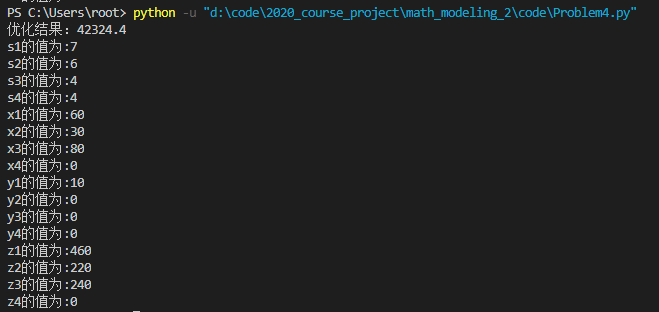
\includegraphics{D:/code/2020_course_project/math_modeling_2/pic/4-1.png}
\caption{}
\end{figure}

即最低总预算为:

\begin{gather*}\sum_{i=0}^{4}w_i=w_0+42324.40=66207.4\end{gather*}

此时各变量的值如上图所示。

\hypertarget{header-n213}{%
\section{2.6 附加问题}\label{header-n213}}

我们对第二个问题进行求解,若每名教练每个月可以指导不超过20名新飞行员(不包括他自己在内)进行训练,则将飞行员和教练分开,即将变量声明中:

\begin{gather*}飞行员中教练和新飞行员数量z_1,z_2,z_3,z_4\end{gather*}

改为:

\begin{gather*}飞行员中教练数量为z_1,z_2,z_3,z_4,新飞行员数量为n_1,n_2,n_3,n_4\end{gather*}

其他符号不改变,则飞行员的数量限制约束变为:

\begin{gather*}第一个月末:z_1+s_1=30 \\第二个月末:z_2+s_2-z_1-s_1-n_1=-450 \\第三个月末:z_3+s_3-z_2-s_2-n_2=-210 \\第四个月末:z_4+s_4-z_3-s_3-n_3=-240 \\其中,n_i<=20z_1\end{gather*}

使用Python的PULP库进行求解,详细代码请参考code文件夹中的Problem4\_2.py。得到结果如下:

\begin{figure}
\centering
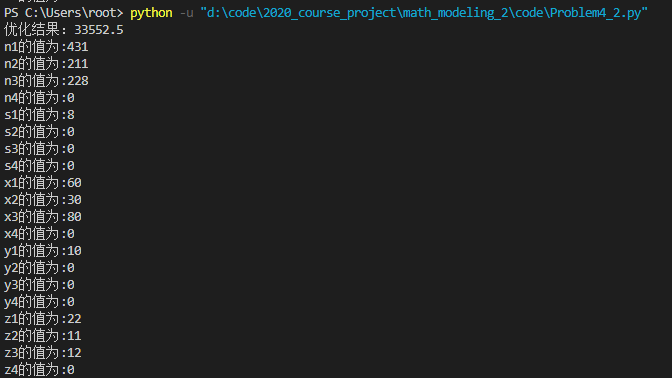
\includegraphics{D:/code/2020_course_project/math_modeling_2/pic/4-2.png}
\caption{}
\end{figure}

即最低总预算为:

\begin{gather*}\sum_{i=0}^{4}w_i=w_0+33552.5=57435.5\end{gather*}

\hypertarget{header-n224}{%
\section{2.7 结果}\label{header-n224}}

通过以上模型结合代码可以求得,问题1的情况下,最低总预算为:

\begin{gather*}\sum_{i=0}^{4}w_i=w_0+42324.40=66207.4\end{gather*}

此时甲方四个月新购飞机数量分别为:\(x_1=60,x_2=30,x_3=80,x_4=0\)

甲方四个月新飞行员和教练数量分别为:\(z_1=460,z_2=220,z_3=240,z_4=0\)

在问题2的情况下,最低总预算为:

\begin{gather*}\sum_{i=0}^{4}w_i=w_0+33552.5=57435.5\end{gather*}

此时甲方四个月新购飞机数量分别为:\(x_1=60,x_2=30,x_3=80,x_4=0\)

甲方四个月新飞行员数量分别为:\(n_1=431,n_2=211,n_3=228,n_4=0\)

\hypertarget{header-n233}{%
\chapter{3 训练题6}\label{header-n233}}
\setcounter{table}{0}\setcounter{figure}{0}
\hypertarget{header-n234}{%
\section{3.1 问题表述}\label{header-n234}}

有若干工厂的污水经排污口流入某江,各口有污水处理站,处理站对面是居民点,工厂1上游江水流量和污水质量浓度、国家标准规定的水的污染浓度及各个工厂的污水流量和污水质量浓度均已知道。设污水处理费用与污水处理前后的质量浓度差和污水流量成正比,使每单位流量的污水下降一个质量浓度单位需要的处理费用(称处理系数)为已知。处理后的污水与江水混合,流到下一个排污口之前,自然状态下的江水也会使污水质量浓度降低一个比例系数(称自净系数),该系数可以估计。试确定各污水处理站出口的污水质量浓度,使在符合国家标准规定的条件下总的处理费用最小。

先建立一般的数学模型,在求解以下的具体问题:

设上游江水流量为\(1000×10^{12}L/min\),污水质量浓度为\(0.8mg/L\),3个工厂的污水流量均为\(5×10^{12}L/min\),污水质量浓度(从上游到下游排列)(单位:mg/L)分别为100,60,50,处理系数均为1万元/(1012L/min)×(mg/L),设3个工厂之间的两段江面的自净系数(从上游到下游)分别为0.9和0.6。国家标准规定水的污染浓度不能超过1mg/L。

\begin{enumerate}
\def\labelenumi{\arabic{enumi}.}
\item
  为了使江面上所有地段的水污染程度达到国家标准,最少需要花费多少费用?
\item
  如果只要求3个居民点上游的水污染程度达到国家标准,最少需要花费多少费用?
\end{enumerate}

\hypertarget{header-n243}{%
\section{3.2 基本假设}\label{header-n243}}

\begin{enumerate}
\def\labelenumi{\arabic{enumi}.}
\item
  仅考虑上游江水及工厂的排水,不考虑其他水流;
\item
  自净系数的估计使较为准确的,可以用于实际计算;
\item
  上游江水污水质量浓度不超过国家标准;
\item
  计算居民点上游的水污染程度时不计算此次汇入的污水。
\end{enumerate}

\hypertarget{header-n253}{%
\section{3.3 变量声明}\label{header-n253}}

\begin{enumerate}
\def\labelenumi{\arabic{enumi}.}
\item
  流经第k个工厂前的江水流量为\(F_k\),污水质量浓度为\(p_k\);
\item
  第k个工厂的污水流量为\(L_k\),污水质量浓度为\(x_k\);
\item
  第k个污水处理厂的处理系数为\(q_k\),经过污水处理后的污水质量浓度为\(y_k\),处理费用为\(w_k\);
\item
  第k个工厂到第k+1个工厂之间这段江水的自净系数为\(r_k\);
\item
  流出第k个工厂后的江水流量为\(G_k\),污水质量浓度为\(u_k\);
\item
  工厂个数为N;
\item
  国家规定的污水质量浓度为\(s\);
\end{enumerate}

\hypertarget{header-n269}{%
\section{3.4 建模思路}\label{header-n269}}

首先考虑一般情况,对于第k个工厂,为保证混合后的江水污水质量浓度符合国家标准,得到:

\begin{gather*}u_k=\frac{F_k\times p_k+L_k\times y_k}{G_k}\leq s\\
G_k=F_k+L_k\end{gather*}

同时得到第k个污水处理厂的费用\(w_k=q_k\times L_k\times (x_k-y_k)\)

对于第k个工厂流入江水的流量和污水质量浓度可以得到下列递推关系:

\begin{gather*}p_k=u_{k-1}\times r_{k-1}\\
F_k=G_{k-1}\end{gather*}

综上,可以得到目标函数

\begin{gather*}min \qquad \sum_{k=1}^Nw_k=\sum_{k=1}^NL_k\times (x_k-y_k)\times q_k\end{gather*}

约束关系:

\begin{gather*}s.t. \qquad u_k=\frac{F_k\times p_k+L_k\times y_k}{F_k+L_k}\leq s\\
y_k\leq x_k\\
p_k=u_{k-1}\times r_{k-1}\\
F_k=F_{k-1}+L_{k-1}\end{gather*}

得到该问题的数学规划模型。

\hypertarget{header-n280}{%
\section{3.5 模型简化}\label{header-n280}}

我们发现上述模型的数学表达式较为复杂,可以在一定程度上进行简化。我们注意到在实际情况中,相比于原本江水的流量,从工厂排出的污水流量是很小的,因此,我们可以认为,污水对于江水流量的影响很小,即江水流量可以视为常数。由此,我们的得到:

\begin{gather*}F_k=G_k=F_1\end{gather*}

将该式带入上述的数学规划模型,我们可以得到一个更加简单的模型:

\begin{gather*}min \qquad \sum_{k=1}^Nw_k=\sum_{k=1}^NL_k\times (x_k-y_k)\times q_k\\
\qquad  \\
s.t. \qquad u_k=\frac{F_1\times p_k+L_k\times y_k}{F_1}=p_k+\frac{L_k \times y_k}{F_1} \leq s\\
0\leq y_k\leq x_k\\
p_k=u_{k-1}\times r_{k-1}\\\end{gather*}

\hypertarget{header-n285}{%
\section{3.6 模型求解}\label{header-n285}}

对于第一问根据题意将数值进行带入:\(F_1=1000\times 10^{12}L/min\),\(p_1=0.8mg/L\),\(L_1=L_2=L_3=5\times 10^{12}L/min\),\(x_1=100mg/L\),\(x_2=60mg/L\),\(x_3=50mg/L\),\(q_1=q_2=q_3=1万元/((10^{12}L/min)\times (mg/L))\),\(r_1=0.9\),\(r_2=0.6\),\(s=1mg/L\)。

得到模型

\begin{gather*}min \qquad 5\times 1\times ((100-y_1)+(60-y_2)+(50-y_3))\\
\qquad  \\
s.t.\qquad 0.8+\frac{5\times 10^{12}\times y_1}{1000\times 10^{12}}=0.8+0.005y_1\leq 1\\
(0.8+0.005y_1)\times 0.9+0.005\times y_2\leq 1\\
((0.8+0.005y_1)\times 0.9+0.005\times y_2)\times 0.6+0.005\times y_3\leq 1\\
0\leq y_1 \leq 100\\
0\leq y_2 \leq 60\\
0\leq y_3 \leq 50\end{gather*}

对于第二问,只需要将\(u_k<s\)改为\(p_k<s\)即可,得到模型

\begin{gather*}min \qquad 5\times 1\times ((100-y_1)+(60-y_2)+(50-y_3))\\
\qquad  \\
s.t.\qquad(0.8+0.005y_1)\times 0.9\leq 1\\
((0.8+0.005y_1)\times 0.9+0.005\times y_2)\times 0.6\leq 1\\
0\leq y_1 \leq 100\\
0\leq y_2 \leq 60\\
0\leq y_3 \leq 50\end{gather*}

\hypertarget{header-n291}{%
\section{3.7 结果}\label{header-n291}}

使用Mathematic计算上述第一问模型

\begin{figure}
\centering
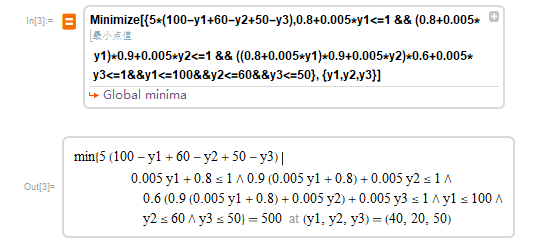
\includegraphics{D:/code/2020_course_project/math_modeling_2/pic/6-1.png}
\caption{}
\end{figure}

得到当\(y_1=40,y_2=20,y_3=50\),即第一个工厂处理浓度为60,第二个工厂处理浓度40,第三个工厂不处理(单位:\(mg/L\)),江面上所有地段水污染达到国家标准且花费取到最小值,最小值为500万元。

计算第二问模型

\begin{figure}
\centering
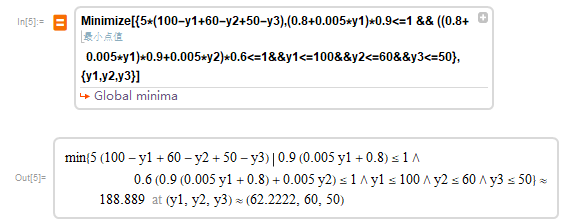
\includegraphics{D:/code/2020_course_project/math_modeling_2/pic/6-2.png}
\caption{}
\end{figure}

得到当\(y_1=62.22,y_2=20,y_3=50\),即第一个工厂处理浓度为38.88,第二个工厂和第三个工厂不处理(单位:\(mg/L\)),三个居民点上游水污染达到国家标准且花费取到最小值,最小值为188.89万元。

\hypertarget{header-n298}{%
\chapter{4 训练题13}\label{header-n298}}
\setcounter{table}{0}\setcounter{figure}{0}
\hypertarget{header-n299}{%
\section{4.1 问题表述}\label{header-n299}}

某农场有3万亩农田(1亩 =
667.67m2),准备种植玉米、大豆和小麦3种农作物,每种作物每亩需施化肥分别为0.12t,0.20t,0.15t。预计秋后玉米每亩可收获500kg,售价为1.2元/kg;大豆每亩可收获200kg,售价为6元/kg;小麦每亩可收获300kg,售价为3.5元/kg。农场年初规划时依次考虑以下几个方面:

(1)年终总收益尽量不低于1650万元

(2)总产量尽量不低于1.25×104t

(3)小麦产量以0.5×104t为宜

(4)大豆产量尽量不低于0.2×104t

(5)玉米产量尽量不超过0.6×104t

(6)农场目前能提供5000t化肥;若不够,可额外购买,但希望额外购买量越少越好。

请为该农场指定种植规划。

\hypertarget{header-n308}{%
\section{4.2 基本假设}\label{header-n308}}

1、农作物的产量预计准确。

2、农作物售价不会发生明显变化。

3、土地、天气等环境因素符合理想化。

\hypertarget{header-n312}{%
\section{4.3 模型建立}\label{header-n312}}

用\(x_1\)、\(x_2\)、\(x_3\)表示该农场种植玉米、大豆、小麦的面积。(单位:亩)

并将各数据填表如下:

\begin{longtable}[]{@{}cccc@{}}
\toprule
种类 & 玉米 & 大豆 & 小麦\tabularnewline
\midrule
\endhead
亩产量(kg) & 500 & 200 & 300\tabularnewline
售价(元/kg) & 1.2 & 6 & 3.5\tabularnewline
肥料(t/亩) & 0.12 & 0.20 & 0.15\tabularnewline
\bottomrule
\end{longtable}

隐藏约束:①\(x_1+x_2+x_3\leq 30000\) ②\(x_1,x_2,x_3\geq0\)

柔性约束(约束强度递减):

(1)年终总收益尽量不低于1650万元:\(x_1\times500\times1.2+x_2\times200\times6+x_3\times300\times3.5\geq 1650\times10^4\)

(2)总产量尽量不低于1.25×104t:\(x_1\times500+x_2\times200+x_3\times300\geq1.25\times10^7\)

(3)小麦产量以0.5×104t为宜:\(x_3\times300= 0.5\times10^7\)

(4)大豆产量尽量不低于0.2×104t:\(x_2\times200\geq0.2\times10^7\)

(5)玉米产量尽量不超过0.6×104t:\(x_1\times500\leq0.6\times10^7\)

(6)农场目前能提供5000t化肥;若不够,可额外购买,但希望额外购买量越少越好:\(x_1\times0.12+x_2\times0.20+x_3\times0.15\leq0.5\;or\;min(x_1\times0.12+x_2\times0.20+x_3\times0.15-0.5)\)

\hypertarget{header-n344}{%
\section{4.4 建模思路}\label{header-n344}}

所以我们得到线性规划模型如下:

求出\(x_1,x_2,x_3\),且满足以下约束:

\(x_1+x_2+x_3\leq 30000\)

\(4x_1+8x_2+7x_3\geq110000\)

\(10x_1+4x_2+6x_3\geq250000\)

\(x_3=\frac{50000}{3};x_2\geq10000;0\leq x_1\leq12000\)

\(12x_1+20x_2+15x_3\leq500000\)

\hypertarget{header-n352}{%
\section{4.5 求解}\label{header-n352}}

利用Lingo对上述模型进行求解,会发现在这几个约束条件内找不到可行解,代码文件见附属文件中的13.1.lg4文件,如下图:

\begin{figure}
\centering
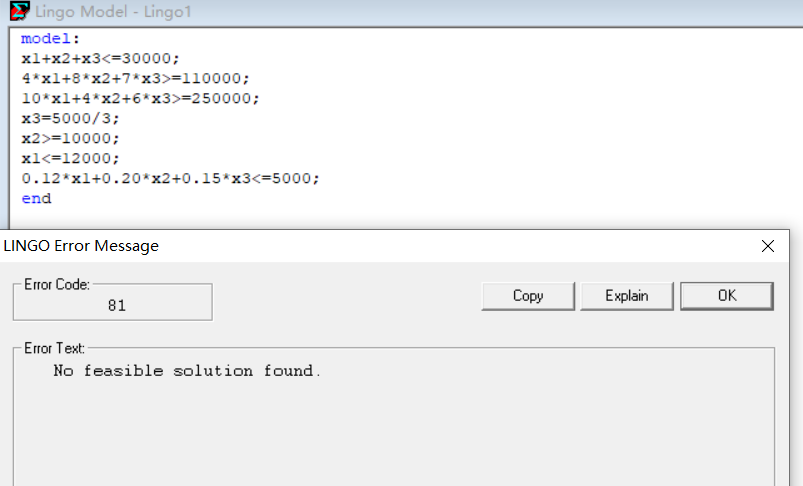
\includegraphics{D:/code/2020_course_project/math_modeling_2/pic/zhk1.png}
\caption{}
\end{figure}

于是需要我们对约束进行一定的放松,根据约束强度把柔性约束从后向前进行放松,即将约束放宽从而尝试能否找到可行解。

于是将所有放宽后的柔性约束连同刚性约束列出如下:

\(x_1+x_2+x_3\leq30000\)

\(max(4x_1+8x_2+7x_3)\)

\(max(10x_1+4x_2+6x_3)\)

\(x_3>=0,x_2>=0,x_1>=0\)

\(min(12x_1+20x_2+15x_3-500000)\)

然后从后往前依次放宽约束,并利用lingo进行求解。

最后可以得到在放宽了\(x_3=\frac{5}{3}\)这个约束条件及其之后的约束条件之后,整个模型就能得到可行解了,代码文件见附属文件中的13.2.lg4文件。即小麦产量以0.5×104t为宜,这一条件及约束强度更低的条件被放宽后,整个模型就有了可行解,且最后一个约束条件可以不用放宽也能得到可行解。如下图:

\begin{figure}
\centering
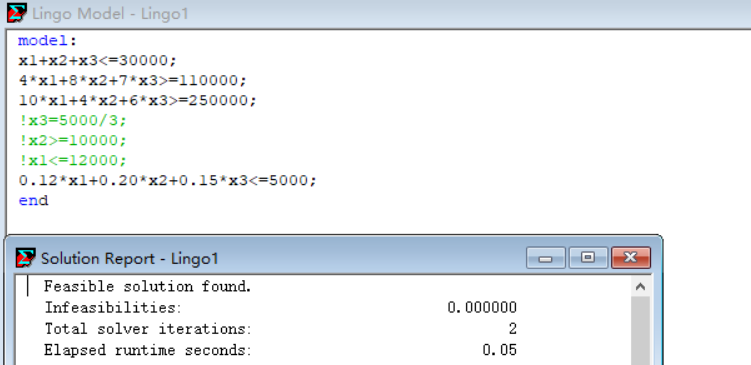
\includegraphics{D:/code/2020_course_project/math_modeling_2/pic/zhk2.png}
\caption{}
\end{figure}

\hypertarget{header-n365}{%
\section{4.6 最终优化求解}\label{header-n365}}

因为需要放宽约束来获得可行解,虽然获得了可行解,但是我们为了利益更大化以及可以适度收紧前面的约束来使放松约束的后遗症达到最小,所以我们在上文放松约束的背景上收紧可以实现的约束来使农场的收益最大化,更改如下:

\(x_1+x_2+x_3=30000\)

\(4x_1+8x_2+7x_3\geq110000\)

\(10x_1+4x_2+6x_3\geq250000\)

\(max(4x_1+8x_2+7x_3)\)

\(max(10x_1+4x_2+6x_3)\)

\(x_3>=0,x_2>=0,x_1>=0\)

\(12x_1+20x_2+15x_3<=500000\)

主要更改即将农场的所有农田用完,然后是在总收入和总产量满足约束的前提下将其变得最大,从而使农场的收益最大。因为这涉及到两个目标函数,我们将采用在总收入最大的前提下,再将总产量变得最大来获得最佳的数据,代码文件见附属文件中的13.3.lg4、13.4.lg4文件。

最终得到数据如下:

\begin{figure}
\centering
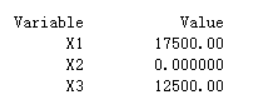
\includegraphics{D:/code/2020_course_project/math_modeling_2/pic/zhk3.png}
\caption{}
\end{figure}

然后根据数据计算出结果即可。

\hypertarget{header-n378}{%
\section{4.7 结果}\label{header-n378}}

\begin{longtable}[]{@{}cc@{}}
\toprule
种类 & 种植面积(亩)\tabularnewline
\midrule
\endhead
玉米 & 17500\tabularnewline
大豆 & 0\tabularnewline
小麦 & 12500\tabularnewline
\bottomrule
\end{longtable}

\begin{longtable}[]{@{}cc@{}}
\toprule
类型 & /\tabularnewline
\midrule
\endhead
总收入 & 157500元\tabularnewline
总产量 & 250000kg\tabularnewline
总化肥 & 3975t\tabularnewline
\bottomrule
\end{longtable}

\hypertarget{header-n405}{%
\chapter{5 参考文献}\label{header-n405}}
\setcounter{table}{0}\setcounter{figure}{0}
{[}1{]}赵伟.谈最优化方法在数学建模中的应用{[}J{]}.数学学习与研究,2020(02):16.

{[}2{]}义欣.基于Matlab和Lingo的线性规划问题求解过程对比分析{[}J{]}.科技视界,2019(17):94-96.

{[}3{]}熊文涛,肖应雄.LINGO软件在目标规划实验教学中的应用{[}J{]}.新疆师范大学学报(自然科学版),2019,38(01):65-69.

\hypertarget{header-n409}{%
\chapter{6 小组分工}\label{header-n409}}
\setcounter{table}{0}\setcounter{figure}{0}
\begin{longtable}[]{@{}ccc@{}}
\toprule
姓名 & 学号 & 分工\tabularnewline
\midrule
\endhead
杨哲宇 & 17376137 & 训练题6,格式排版\tabularnewline
杨壮 & 17376193 & 训练题4,格式排版\tabularnewline
叶天宇 & 18373729 & 训练题2\tabularnewline
张涵珂 & 18373734 & 训练题13\tabularnewline
蔡星辰 & 18373734 & 摘要,引言,参与讨论\tabularnewline
\bottomrule
\end{longtable}

\end{document}
